%%%%%%%%%%%%
%
% $Autor: Wings $
% $Datum: 2019-03-05 08:03:15Z $
% $Pfad: Functions.tex $
% $Version: 4250 $
% !TeX spellcheck = en_GB/de_DE
% !TeX encoding = utf8
% !TeX root = manual 
% !TeX TXS-program:bibliography = txs:///biber
%
%%%%%%%%%%%%

\chapter{Functions}

\section{Functions}

This section provides a detailed description of each primary function in the \textbf{License Plate Detection System}. 
Each function contributes to the end-to-end workflow—from video capture to recognition and logging—operating efficiently on the NVIDIA Jetson Nano platform.

% ==========================================================
\subsection{Function 1: Live Video Capture}
\textbf{Purpose:} Acquire live video frames from the Microsoft LifeCam Show via USB and prepare them for inference.

\textbf{Description:}
\begin{itemize}
	\item Utilizes OpenCV’s \texttt{cv2.VideoCapture()} for frame streaming.
	\item Converts BGR to RGB format for compatibility with YOLOv8.
	\item Maintains stable FPS by adjusting camera exposure dynamically.
\end{itemize}

\begin{figure}[h!]
	\centering
	\begin{tikzpicture}[>=stealth, thick]
		\tikzstyle{io}=[ellipse, draw=gray!70!black, fill=gray!10, minimum height=1cm, text centered, text width=3.5cm]
		\tikzstyle{block}=[rectangle, draw=blue!70!black, fill=blue!10, rounded corners, minimum height=1cm, text width=4cm, text centered]
		\tikzstyle{output}=[ellipse, draw=green!70!black, fill=green!10, text width=2.5cm, text centered]
		
		\node[io] (input) at (0,0) {\faCamera\\Camera Feed};
		\node[block] (process) at (5,0) {OpenCV\\Frame Capture + RGB Conversion};
		\node[output] (output) at (10,0) {Processed Frames\\(640×480 RGB)};
		
		\draw[->, thick] (input) -- node[above]{} (process);
		\draw[->, thick] (process) -- node[above]{} (output);
	\end{tikzpicture}
	\caption{Live video capture and preprocessing.}
	\label{fig:video_capture}
\end{figure}

% ==========================================================
\subsection{Function 2: License Plate Detection (YOLOv8)}
\textbf{Purpose:} Detect and localize license plates in each frame using a YOLOv8-Nano model optimized for Jetson Nano GPU inference.

\textbf{Description:}
\begin{itemize}
	\item Loads trained YOLOv8 model weights (\texttt{best.pt}).
	\item Runs real-time inference (~13–15 FPS) via TensorRT optimization.
	\item Returns bounding boxes and confidence scores for each detected plate.
\end{itemize}

\begin{figure}[h!]
	\centering
	\begin{tikzpicture}[>=stealth, thick]
		\tikzstyle{img}=[rectangle, draw=gray!60!black, fill=gray!10, text width=3.3cm, align=center, minimum height=1cm]
		\tikzstyle{block}=[rectangle, draw=green!60!black, fill=green!10, rounded corners, text centered, text width=3.5cm, minimum height=1cm]
		\tikzstyle{annot}=[text width=2.2cm, align=center, font=\small]
		
		\node[img] (input) at (0,0) {Input Frame};
		\node[block] (yolo) at (5,0) {YOLOv8 Detection Engine};
		\node[img] (output) at (10,0) {Detected Plates\\(Bounding Boxes)};
		\node[annot] (gpu) at (5,1.8) {\faMicrochip\\GPU Inference};
		
		\draw[->, thick] (input) -- node[above]{\scriptsize Data} (yolo);
		\draw[->, thick] (yolo) -- node[above]{} (output);
		\draw[dashed, ->, gray!70] (gpu) -- (yolo);
	\end{tikzpicture}
	\caption{YOLOv8 model performing plate detection on Jetson Nano GPU.}
	\label{fig:yolo_function}
\end{figure}

% ==========================================================
\subsection{Function 3: Optical Character Recognition (EasyOCR)}
\textbf{Purpose:} Convert detected license plate regions into machine-readable text.

\textbf{Description:}
\begin{itemize}
	\item Crops bounding box regions and preprocesses them (grayscale, thresholding).
	\item Uses EasyOCR to extract alphanumeric characters.
	\item Returns recognized text and confidence score for logging.
\end{itemize}

\begin{figure}[h!]
	\centering
	\begin{tikzpicture}[>=stealth, thick]
		\tikzstyle{block}=[rectangle, draw=blue!70!black, fill=blue!10, rounded corners, text centered, text width=4cm, minimum height=1cm]
		\tikzstyle{stage}=[ellipse, draw=orange!80!black, fill=orange!10, text width=3.5cm, align=center, minimum height=1cm]
		
		\node[block] (input) at (0,0) {Detected Plate Image};
		\node[stage] (ocr) at (5,0) {EasyOCR Recognition};
		\node[block] (output) at (10,0) {Recognized Text + Confidence};
		
		\draw[->, thick] (input) -- node[above]{} (ocr);
		\draw[->, thick] (ocr) -- node[above]{} (output);
	\end{tikzpicture}
	\caption{EasyOCR text extraction workflow.}
	\label{fig:ocr_function}
\end{figure}

% ==========================================================
\subsection{Function 4: Database Logging (SQLite)}
\textbf{Purpose:} Store recognized license plate data with timestamps into a structured local database.

\textbf{Description:}
\begin{itemize}
	\item Uses Python’s \texttt{sqlite3} to manage \texttt{plates.db}.
	\item Ensures unique entries to prevent duplicates.
	\item Allows quick query for analysis or export.
\end{itemize}

\begin{figure}[h!]
	\centering
	\begin{tikzpicture}[>=stealth, thick]
		\tikzstyle{block}=[rectangle, draw=purple!70!black, fill=purple!10, rounded corners, text centered, text width=3.5cm, minimum height=1cm]
		\tikzstyle{db}=[cylinder, shape border rotate=90, draw=orange!90!black, fill=orange!10, 
		minimum height=1.3cm, minimum width=1cm, aspect=0.4, align=center]
		
		\node[block] (input) at (0,0) {Recognized Plate Data};
		\node[block] (sql) at (5,0) {SQLite Interface};
		\node[db] (database) at (10,0) {plates.db};
		
		\draw[->, thick] (input) -- node[above]{\scriptsize Query} (sql);
		\draw[->, thick] (sql) -- node[above]{\scriptsize Stored Record} (database);
	\end{tikzpicture}
	\caption{Data storage using SQLite.}
	\label{fig:db_function}
\end{figure}

% ==========================================================
\textbf{Purpose:} Display live recognition results and handle exception vehicles such as ambulances and police.

\textbf{Description:}
\begin{itemize}
	\item Displays live annotated feed using OpenCV.
	\item Filters out exempt vehicles via JSON list.
	\item Provides real-time alerts on the screen.
\end{itemize}

\begin{figure}[h!]
	\centering
	\begin{tikzpicture}[>=stealth, thick]
		\tikzstyle{block}=[rectangle, draw=gray!70!black, fill=gray!10, rounded corners, text width=3.5cm, align=center, minimum height=1cm]
		\tikzstyle{json}=[diamond, aspect=2.2, draw=orange!80!black, fill=orange!10, text centered, text width=3cm]
		\tikzstyle{output}=[ellipse, draw=blue!70!black, fill=blue!10, text width=3.5cm, align=center, minimum height=1cm]
		
		\node[block] (input) {YOLO + OCR Results};
		\node[json, below left=1.2cm and -0.2cm of input] (filter) {Exception\\Check (JSON)};
		\node[output, below right=1.2cm and -0.2cm of input] (display) {Final Display / Alert};
		
		\draw[->, thick, bend right=20] (input) to node[left]{\scriptsize Vehicle ID} (filter);
		\draw[->, thick, bend left=20] (input) to node[right]{\scriptsize Display Data} (display);
		\draw[->, thick, dashed, orange!80!black] (filter) to node[below]{} (display);
	\end{tikzpicture}
	\caption{Non-linear display and filtering logic.}
	\label{fig:display_function}
\end{figure}

% ==========================================================
\subsection*{Summary of Functional Modules}
\begin{table}[h!]
	\centering
	\caption{Functional Overview Summary}
	\begin{tabular}{|l|l|l|}
		\hline
		\textbf{Function} & \textbf{Primary Tool/Library} & \textbf{Output Type} \\ \hline
		Video Capture & OpenCV & Frame stream (RGB) \\ \hline
		Detection & YOLOv8 & Bounding boxes + Confidence \\ \hline
		Recognition & EasyOCR & Alphanumeric Text \\ \hline
		Database & SQLite3 & Structured Records \\ \hline
		Display & OpenCV + JSON & Annotated Feed \\ \hline
	\end{tabular}
\end{table}
